%! TEX root = ../thesis.tex
\section{Deployed System}%
\label{pdk:sec:depsys}

We deploy a Web platform, called Predikon\footnote{The platform is available on \href{http://www.predikon.ch}{www.predikon.ch}.}, to provide real-time predictions for Swiss referenda (see Appendix~\ref{app:sec:predikon}.
Four Sundays a year, Swiss citizens are called on to vote on at least one item in a referendum.
These items can cover a broad range of topics, from joining the European Union to subsidizing railways and roads, from banning the use of fossil fuels to cutting taxes, and even forbidding Swiss farmers to remove horns from cows and goats.
A month prior to a referendum vote day, eligible voters receive official ballots, together with useful documentation.
To cast their vote, they can either send their ballot by post or bring it to the ballot office on the referendum vote day, up to 11:59am.
Starting at 12pm, each municipality is in charge of counting both the remote ballots and the ballots they collected on the same day.
Once they have finished counting, they report the result to their canton whose administration communicates the official count.

\subsection{Implementation Details}

In 2019, the Swiss Federal Statistical Office released a public API to access vote data, both historical and real-time, for all municipalities in a standardized format~\cite{confederation2020open}.
This enabled us to obtain sequential results in all municipalities on the referendum vote days and made it possible to use our algorithm to predict the outcome of referenda starting at 12pm.
We use the dataset described in Table~\ref{pdk:tab:datasets} for Switzerland, which contains~$R = 2196$ municipalities.
We predict the outcome of twelve items between February 9, 2020, and March 7, 2021.
We summarize these items in Table~\ref{pdk:tab:real_votes}.
On average, the turnout is 53.3\% and 2.8 million valid ballots are counted for each referendum.

\begin{table}
	\centering
	\caption{
		True outcome $y^*_{\textrm{nat}}$, earliest prediction $y_{\textrm{nat}}$, and absolute difference $\Delta = \vert y^*_{\textrm{nat}} - y_{\textrm{nat}} \vert $ for referenda with real data.
	}
	\label{pdk:tab:real_votes}
	\begin{tabular}{llrrr}
		\toprule
		Date         & Item                                & $y^*_{\textrm{nat}}$ [\%] & $y_{\textrm{nat}}$ [\%] & $\Delta$ \\
		\midrule

		Feb 9, 2020  & More Affordable Housing             & 42.97                     & 41.57                   & 1.40     \\
		             & Ban of Sexual Discrimination        & 63.03                     & 62.95                   & 0.08     \\
		Sep 27, 2020 & Moderate Immigration                & 38.35                     & 38.53                   & 0.18     \\
		             & Hunting Act                         & 48.07                     & 47.54                   & 0.53     \\
		             & Tax Deduction of Childcare Expenses & 36.77                     & 35.58                   & 1.19     \\
		             & Paternity Leave                     & 60.27                     & 59.33                   & 0.94     \\
		             & New Fighter Aircrafts               & 50.16                     & 51.29                   & 1.13     \\
		Nov 29, 2020 & Responsible Businesses              & 50.73                     & 50.13                   & 0.60     \\
		             & Ban on Financing War Material       & 42.55                     & 41.91                   & 0.64     \\
		Mar 7, 2021  & Ban on Full Face Coverings          & 51.21                     & 50.80                   & 0.41     \\
		             & e-ID Act                            & 35.64                     & 38.03                   & 2.39     \\
		             & Trade Agreement with Indonesia      & 51.65                     & 51.54                   & 0.11     \\

		\bottomrule
	\end{tabular}
\end{table}

For a vote~$V+1$, we use the historical data up to vote~$V$ to learn the feature matrix~$\vX$ from the sub-matrix~$\vY_V$.
For example, for February 9, 2020, we train the model using~$V = 328$ votes and we predict the results of the two referenda on that date.
We use a Bernoulli likelihood to define our GLM with~$D=25$ latent dimensions and a regularization factor~$\lambda=0.01$.
We fetch municipal results from the API every minute\footnote{Schedule suggested by the Swiss Federal Statistical Office.}.
If new results are available, we learn the optimal parameters~$\vw_*$ by optimizing the negative log-likelihood using Newton's method, and we predict the unobserved municipal results as $\vy_{V+1}^{(\Ubs)} = \sigma(X^{(\Ubs)} \vw_*)$.
Similar to Equation~\eqref{pdk:eq:prediction}, we predict the national outcome~$y_{\textrm{nat}} \in [0, 1]$ by aggregating our prediction of unobserved results~$\Ubs$ with the observed results~$\Obs$ as
\begin{equation*}
	y_{\textrm{nat}} = \frac{1}{N} \left( \sum_{r \in \Ubs} N_r^{(\Ubs)} y_{r, V+1}^{(\Ubs)} + \sum_{r \in \Obs} N_r^{(\Obs)} y_{r, V+1}^{(\Obs)} \right),
\end{equation*}
where~$N_r^{(\Ubs)}$ is the number of valid ballots in municipality~$r$ from the previous vote (used as proxy for the current vote),~$N_r^{(\Obs)}$ is the number of valid ballots in municipality~$r$ for the current vote, and~$N = \sum_{r \in \Ubs} N_r^{(\Ubs)} + \sum_{r \in \Obs} N_r^{(\Obs)}$ is the total number of valid ballots.
As the number of unobserved results~$\vert \Ubs \vert$ tends to 0 with time and the number of observed results~$\vert \Obs \vert$ tends to the total number of regions~$R$, the prediction for the national outcome~$y_{\textrm{nat}}$ converges to the true outcome~$y_{\textrm{nat}}^* \in [0, 1]$.

\subsection{Real-Time Predictions}

In Figure~\ref{pdk:fig:predictions}, we show eight examples of the evolution of our predictions (red line), together with the weighted averaging (black line), as a function of the progress of the ballot counting.
The ballot counting starts at 12pm and ends later in the afternoon, after all municipalities reported their results.
Looking at the trajectory of the weighted averaging, the jumps occurring at several steps correspond to the publication of the results of whole cantons, such as Wallis, and of large municipalities, such as the cities of Basel, Genera, Bern or Zurich.

Our first predictions are made at 12:01pm, using the results of 355 municipalities on average (16.2\% of all municipalities) representing 6.5\% of the total population.
For the twelve referenda, these predictions reach a mean absolute error of 0.8\% to the true outcome.
The largest error is made on the ``e-ID Act'', with a MAE of 2.39\%.
This could be due to the lack of historical votes related to digitalization in Switzerland leading to a vote embedding lying in an empty region of the ideological space.
The weighted average for the current count varies up to a difference of 7.3\%, whereas our predictions are qualitatively stable over time.
To provide a robust estimation of the final outcome, our algorithm takes advantage of the correlation across municipalities and votes.
Furthermore, our earliest predictions were always on the correct side of the 50\% threshold, \textit{i.e.}, it reached an accuracy of 100\% at predicting the acceptance or rejection of a referenda.

\begin{figure}
	\centering
	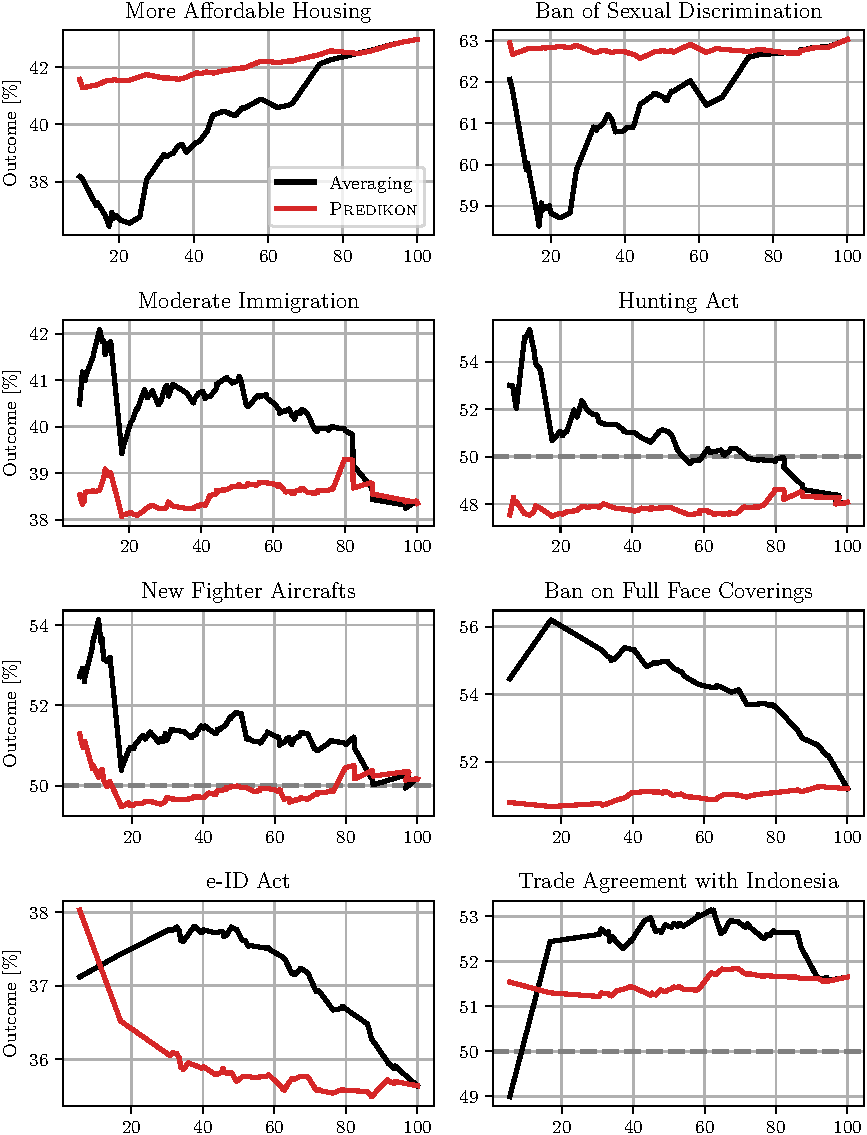
\includegraphics{pdk-predictions.pdf}
	\caption{
		Examples of evolution of predictions (red) and weighted averaging (black) on real, sequential data for the referenda between February 9, 2020, and March 7, 2021.
	}
	\label{pdk:fig:predictions}
\end{figure}
